\section{Evaluation plan}

\subsection{Preliminary Virtualization Results}

\begin{figure}[tbh]
\centering
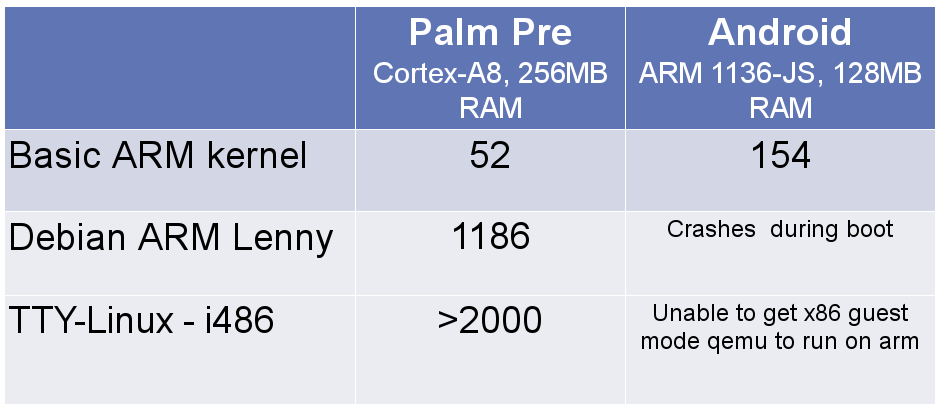
\includegraphics[width=1.0\columnwidth]{virtualization_results}
\caption{Virtualization Results: Kernel Boot time in seconds}
\label{fig:virt_results}
\end{figure}

Currently, virtualization has been tested with QEMU-based implementations running various linuxes on both the Android and the Pre \ref{virt_results}.  The most successful implementation used ARM on ARM virtualization and a basic ARM kernel image provided by QEMU.  Unfortunately, even this implementation was far too slow, taking 52 seconds to boot on the Pre and 154 seconds to boot on the Android.  Additionally response times were terrible, often taking several seconds to display text input.  A Debian ARM Lenny image took over 15 minutes to boot on the Pre and crashed on the Android during boot.  X86 on ARM was also tested, with a TTY-Linux image; however, this was the slowest by far, taking over half an hour to boot on the Pre.  On the Android, x86 guest mode QEMU would not even run.

\subsection{X-Server numbers}

\begin{figure}[tbh]
\centering
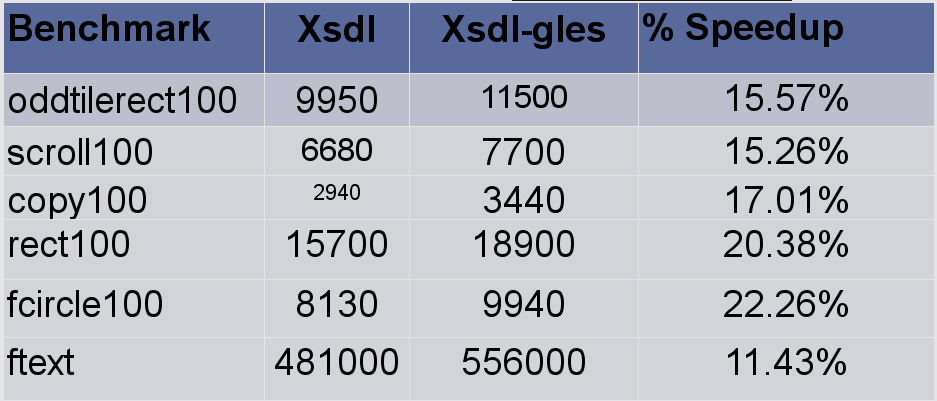
\includegraphics[width=1.0\columnwidth]{x_results}
\caption{X server rendering with x11perf}
\label{fig:x_results}
\end{figure}
